\section{Introduction} % (fold)
\label{sec:Introduction}
In this mini project we study reflective subcategories and their properties. To motivate this a little bit, consider the category of abelian groups which are contained in the category of groups. The abelianization functor then serves as a left adjoint to this inclusion. We can then consider the monad induced by this adjunction and ask ourselves if the category of $ T $-algebras on groups ($ T $ being the monad) is equivalent to the category of abelian groups. As we shall see, this is indeed the case, and it follows from the result that the inclusion of a reflective subcategory is monadic.

We\footnote{``We'' is used only as a literary device, as this is solely my own work.} have chosen to answer the questions that accompany this mini project as an extended text which we have tried to fit together in a logical manner. Section~\ref{sec:Preliminaries} answers questions 1--4 while section~\ref{sec:Monadic Structure of Reflective Subcategories} answers question 5. More specifically, we have the map between questions and theorems/propositions/lemmas as shown in Figure~\ref{fig:map}.
\begin{figure}[ht]
  \begin{center}
    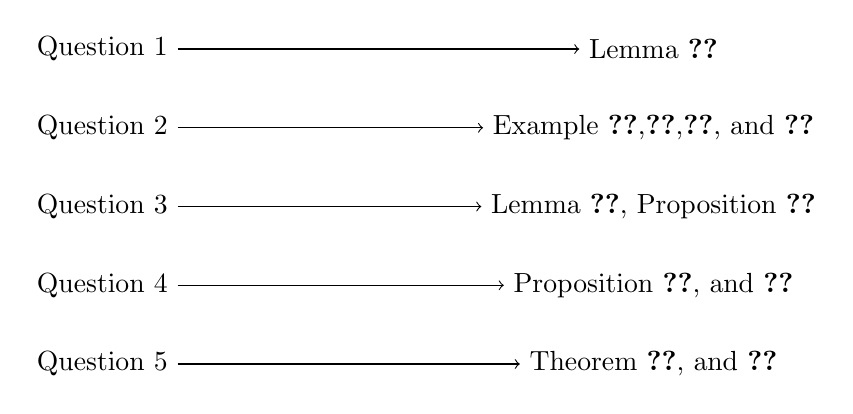
\begin{tikzpicture}
      \node (Q1) at (0,4) {Question 1};
      \node (Q2) at (0,3) {Question 2};
      \node (Q3) at (0,2) {Question 3};
      \node (Q4) at (0,1) {Question 4};
      \node (Q5) at (0,0) {Question 5};
      \node (A1) at (7,4) {Lemma~\ref{lem:adjprops}};
      \node (A2) at (7,3) {Example~\ref{ex:ab},\ref{ex:ring},\ref{ex:met}, and \ref{ex:haus}};
      \node (A3) at (7,2) {Lemma~\ref{lem:ess}, Proposition~\ref{prop:local}};
      \node (A4) at (7,1) {Proposition~\ref{prop:creates}, and~\ref{prop:colims}};
      \node (A5) at (7,0) {Theorem~\ref{thm:beck}, and~\ref{thm:converse}};
      \draw[->] (Q1) -- (A1);
      \draw[->] (Q2) -- (A2);
      \draw[->] (Q3) -- (A3);
      \draw[->] (Q4) -- (A4);
      \draw[->] (Q5) -- (A5);
      % Add more nodes and arrows as needed
    \end{tikzpicture}
  \end{center}
  \caption{Correspondence between questions in the mini project problem sheet and the appropriate results in this text.}\label{fig:map}
\end{figure}

% section Introduction (end)
